\multiproblem{0}{
  Consider this simple truss
  \newline
  \begin{center}
  \includegraphics[scale=1.5]{triangle.pdf}
  \end{center}
  \begin{enumerate}
    \item{ First analyse the general situation of the truss. What are the
      external forces on the truss? What reaction forces could there be at the
      supports? How many unknown reaction forces are there for the truss as a
      whole? Draw a free body diagram showing the truss and the external
      forces applied to it.\A{ \\
Firstly, we need to know what external forces are acting on the truss as a whole. There is clearly a horizontal force exerted at point $B$ of 2 kN. The pin joint at $A$ can also exert a force on the truss with both horizontal and vertical components, as the joint allows no translation. At point $C$ the roller joint allows horizontal translation and so it can only exert a vertical force. So, we can draw these forces on our diagram.
 \begin{center}
    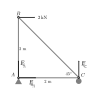
\includegraphics[scale=1.5]{triangle_soln_1.pdf}
  \end{center}
To simplify the diagram let us draw the truss a particle for our free body force diagram.
 \begin{center}
    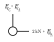
\includegraphics[scale=1.5]{triangle_soln_2.pdf}
  \end{center}
}}
    \item{ Use force and moment balance for the truss as a whole to find all
      the external reaction forces.\A{Since the truss is in static equilibrium leads us to the following equations:
$F_{V_C}+F_{V_A}=0$ and $F_{H_A}+2$ kN $=0$
 \begin{center}
    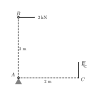
\includegraphics[scale=1.5]{triangle_soln_3.pdf}
  \end{center}
Taking moment about point $A$ we find that $2 \times 2$ kN $ - 2 \times F_{V_{C}}=0$ and so clearly $F_{V_{C}}=2$ kN. Using our vertical force balance we can now find that $F_{V_{A}}=-2$ kN.
}}
    \item{ Redraw the diagram for the truss with the values of the reaction
      forces and label the tensions in each rod as $T_{AB}$, $T_{BC}$ and
      $T_{AC}$. Now use the method of joints (force balance at each joint) to
      find the tensions in each of the rods.\A{\\
We can redraw the daigram with the values of the reaction forces added
 \begin{center}
    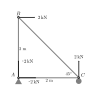
\includegraphics[scale=1.5]{triangle_soln_4.pdf}
  \end{center}
Which is perhaps more clear when we draw all forces in their ``positive'' direction.
 \begin{center}
    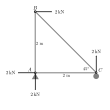
\includegraphics[scale=1.5]{triangle_soln_5.pdf}
  \end{center}
With the external forces found we can now analyse each joint.
 \begin{center}
    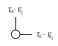
\includegraphics[scale=1.5]{triangle_soln_A.pdf}
  \end{center}
Clearly, $T_{AB}+F_{V_{A}}=0$, so $T_{AB}=2$ kN.  $T_{AC}+F_{H_{A}}=0$, so $T_{AC}=2$ kN.
 \begin{center}
    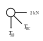
\includegraphics[scale=1.5]{triangle_soln_B.pdf}
  \end{center}
For point $B$ we have $T_{AB}+T_{BC}\mathrm{sin}(45)=0$, and $2$ kn $+T_{BC}\mathrm{sin}(45)=0$ from which it is easy to find that $T_{BC}=-2/ \mathrm{sin}(45)$ kN.
 \begin{center}
    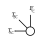
\includegraphics[scale=1.5]{triangle_soln_C.pdf}
  \end{center} 
At point $C$ we can find that $T_{AC}+T_{BC}\mathrm{sin}(45)=0$ and $F_{V_{C}}+T_{BC}\mathrm{sin}(45)=0$. Therefore, $T_{BC}=-2/ \mathrm{sin}(45)$ kN. }}
  \end{enumerate}
}

\multiproblem{0.1}{
  Use the method of joints to find all reaction forces and tensions in this
  structure:
  \begin{center}
    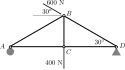
\includegraphics[scale=1.5]{mj_1.pdf}
  \end{center}
.\A{\\
We can begin by looking at the joints at $A$ and $D$ at what kind of forces they can exert. The possible external forces are shown in the following figure.
 \begin{center}
    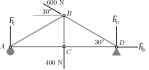
\includegraphics[scale=1.5]{mj_1_soln_1.pdf}
  \end{center}
Treating the truss as a single particle we can draw a free body force diagram. From this we can find the vertical and horizontal force balance equations. $F_{V_{A}}+F_{V_{D}} - 400$ kN $ -  600\mathrm{sin}(30)$ kN $=0$ and $F_{V_{D}}+ 600 \mathrm{cos}(30)$ kN $=0$. Immediately, we know that  $F_{V_{D}}=- 600 \mathrm{cos}(30)$ kN $=0$.
 \begin{center}
    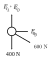
\includegraphics[scale=1.5]{mj_1_soln_2.pdf}
  \end{center}
Let us now look at the moments. It is perhaps easiest to take these about $D$. If we take the lengths $AC$ (and $CD$) to be $L$. The moment balance gives $2L\times F_{A_{V}}-L \times 400$ kN $=0$. For this, we find that $F_{A_{V}}=200$ kN. Substituting this result into our previous equations we can find  $F_{V_{D}}=  400$ kN $ +  600\times \mathrm{sin}(30)$ kN $- 200$ kN.
 \begin{center}
    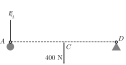
\includegraphics[scale=1.5]{mj_1_soln_3.pdf}
  \end{center}
Now, since we have found the external forces we can now investiagte each joint. Starting with joint $A$ we find that $F_{V_{A}}+T_{AB}\mathrm{sin}(30)=0$, and so $T_{AB}=-200/\mathrm{sin}(30)$ kN. Furthermore, we can find that $T_{AB}\mathrm{cos}(30) + T_{AC}=0$ and so $T_{AC}=200 \mathrm{cot}(30)$ kN.
 \begin{center}
    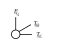
\includegraphics[scale=1.5]{mj_1_soln_A.pdf}
  \end{center}
Now, looking at point $B$: $T_{AB} \mathrm{cos}(30)=(T_{BD}+600) \mathrm{cos}(30)$. From which we can find $T_{BD}=(T_{AB}-600)=-600 -200/\mathrm{sin}(30)$ kN. We could find $T_{BC}$ from the vertical balance at $B$. However, it perhaps easier to find this from the vertical balance at $C$.
 \begin{center}
    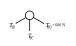
\includegraphics[scale=1.5]{mj_1_soln_B.pdf}
  \end{center}
The force balance equations are simple to find: $T_{BC}-400$ kN $=0$ and $T_{CD}-T_{AC}=0$. Therefore, $T_{BC}=400$ kN and $T_{CD}=200 \mathrm{cot}(30)$ kN.
 \begin{center}
    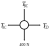
\includegraphics[scale=1.5]{mj_1_soln_C.pdf}
  \end{center} }
}

\multiproblem{0.2}{
  Now consider this larger structure:
  \begin{center}
    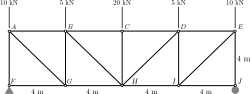
\includegraphics[scale=1.5]{mj_5.pdf}
  \end{center}
  \begin{enumerate}
    \item Use the method of joints to find all tensions and reaction forces in the truss. \AA{\\
    Firstly we find the overall force and moment balance equations. Vertically we have$$F_{F_V}+F_{J_V}=50\,\mathrm{kN}.$$
	Furthermore, if we take moments about $H$ we can easily find that $F_{F_V}+F_{J_V}$. It is also easy to find that $F_{F_H}=0$ from the horizontal force balance.}
    \item Use the method of sections to calculate $T_{BC}$,
      $T_{BH}$, $T_{GH}$ (hopefully finding the same answer as before\ldots)\AA{\\
      \begin{center}
      		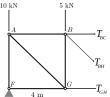
\includegraphics[scale=1.5]{mj_5_sec.pdf}
      \end{center} }
  \end{enumerate}
}

\multiproblem{0.3}{
  Use the method of sections to find $T_{BC}$, $T_{CE}$ and $T_{EF}$ in the
  following truss:
  \newline
  \begin{center}
    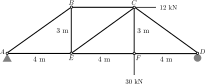
\includegraphics[scale=1.5]{ms_1.pdf}
  \end{center}\A{\\
 \begin{center}
    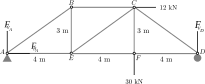
\includegraphics[scale=1.5]{ms_1_soln_1.pdf}
  \end{center}
 \begin{center}
    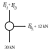
\includegraphics[scale=1.5]{ms_1_soln_2.pdf}
  \end{center}
 \begin{center}
    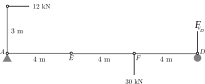
\includegraphics[scale=1.5]{ms_1_soln_3.pdf}
  \end{center}
 \begin{center}
    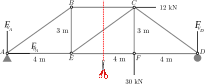
\includegraphics[scale=1.5]{ms_1_soln_4.pdf}
  \end{center}
 \begin{center}
    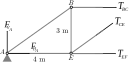
\includegraphics[scale=1.5]{ms_1_soln_5.pdf}
  \end{center}
}
}

\multiproblem{0.4}{
  Find $T_{BH}$ and $T_{CG}$. \hfill
  \begin{center}
    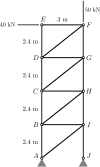
\includegraphics[scale=1.5]{ms_3.pdf}
  \end{center}
}

%\multiproblem{1}{
%  By using the Method of Joints, solve for the support forces
%  and the tension/compression in each rod in the following truss structures:
%  \begin{enumerate}
%    \item Roof Truss: \hfill
%      \begin{center}
%        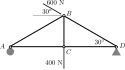
\includegraphics[scale=2]{mj_1.pdf}
%      \end{center}
%    \item Howe Roof Truss: \hfill
%      \begin{center}
%        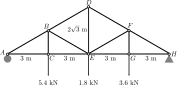
\includegraphics[scale=2]{mj_2.pdf}
%      \end{center}
%    \item Pratt Roof Truss: \hfill
%      \begin{center}
%        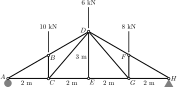
\includegraphics[scale=2]{mj_3.pdf}
%      \end{center}
%    \item \hfill
%      \begin{center}
%        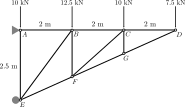
\includegraphics[scale=2]{mj_4.pdf}
%      \end{center}
%    \item \hfill
%      \begin{center}
%        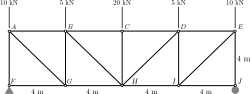
\includegraphics[scale=2]{mj_5.pdf}
%      \end{center}
%      Hint: use symmetry to save calculation time.
%  \end{enumerate}
%}

\multiproblem{best}{
  Suppose we want to make a roof and need to choose a truss type. We consider
  three options: the simple roof truss, the Howe Roof truss and the Pratt Roof
  truss, as shown below. The rods that make the truss can support a given
  maximum tension/compression, denoted $T_{\text{max}}$. If the tension in any
  rod exceeds $\pm T_{\text{max}}$ then the rod is expected to fail (break).
  We want our roof truss to support a load $W$ at the central section (without
  breaking!).\newline
  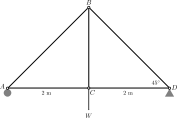
\includegraphics[scale=1.4]{roof.pdf}
  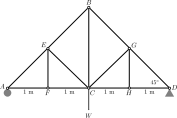
\includegraphics[scale=1.4]{howe.pdf}
  \begin{center}
    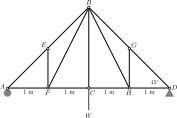
\includegraphics[scale=1.4]{pratt.pdf}
  \end{center}
  \begin{enumerate}
    \item Find the tension in each rod in each truss as a function of the load
      $W$.
    \item Which truss style supports the largest load $W$ if $T_{\text{max}}$
      is the same in each case?
    \item Suppose that we want to minimise the cost of the materials for our
      roof truss while ensuring that is can still support a maximum load
      $W_{\text{max}}$. The cost depends on the length of the truss rods and
      their thickness (which determines their strength). Suppose the cost is
      given by $|T_{\text{max}}|L$ where $L$ is the total length of all truss
      rods and $T_{\text{max}}$ is the maximum tension/compression found in
      the truss under the load $W_{\text{max}}$. Which truss will be cheapest?
  \end{enumerate}

}

% \multiproblem{2}{
% The Method of Sections allows us to find the forces in specific rods more efficiently. It is generally a good idea to cut the truss through the rods with unknown forces.
%     \begin{enumerate}
%         \item Using the Method of Sections:
%         \begin{enumerate}
%         \item Verify the value of $T_{BD}$ and $T_{BE}$ for the truss in 1 (b).
%         \item Verify the value of $T_{DG}$ for the truss in 1 (c).
%         \item Verify your values for $T_{CF}$ and $T_{BC}$ for the truss in 1 (d). 
%         \item Verify your values for $T_{BC}$, $T_{BH}$ and $T_{GH}$ for the truss in 1 (e). 
%         \end{enumerate}
%         \item Find $T_{BC}$, $T_{CE}$ and $T_{EF}$. \hfill
%         \begin{center}
%         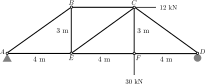
\includegraphics[scale=2]{ms_1.pdf}
%         \end{center}
%         \item Find $T_{BD}$, $T_{BE}$ and $T_{CE}$. \hfill
%         \begin{center}
%         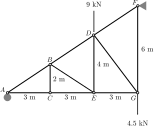
\includegraphics[scale=2]{ms_2.pdf}
%         \end{center}
%         \item Find $T_{BH}$ and $T_{CG}$. \hfill
%         \begin{center}
%         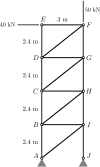
\includegraphics[scale=2]{ms_3.pdf}
%         \end{center}               
%         \item Find $T_{DF}$, $T_{FG}$ and $T_{GI}$. (Hint: Identify all zero-force rods before you make the cut. The easiest way to find these is to begin by considering the force balance at joint $K$.) \hfill
%         \begin{center}
%         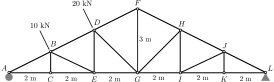
\includegraphics[scale=2]{ms_4.pdf}
%         \end{center}        
%     \end{enumerate}
% }

\multiproblem{3}{
  We would like to build a bridge across a ravine. The truss structure of the
  bridge is as shown below. The truss can be thought of as comprising of $2N$
  sub-structures of width $l$ - for instance, in the bridge below $N=3$. The
  length of the bridge is therefore given by $d=2Nl$.
  \begin{center}
    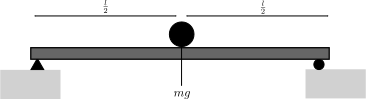
\includegraphics[scale=1.4]{bridge.pdf}
  \end{center} 
  \begin{enumerate}
    \item Using any method you choose find the tension/compression in each rod
      as a function of $W$ for the bridge shown above. (It might be a bit
      easier to use Method of Sections.)
    \item Now consider the general case, where the bridge is composed of $N$
      sub-structures. By using the Method of Sections, find
      tension/compression in each rod as a function of $N$ and $W$.
    \item The maximum tension in any rod is denoted $T_{\text{max}}$. By
      considering the largest load $W$ that can be supported for a given
      $T_{\text{max}}$ for different $N$, show that the strongest truss
      structure for the bridge is the simple Roof Truss.
    \item Suppose that the cost of the bridge is directly proportional to the
      total length of the rods used. Show that for a bridge of length $d$ the
      total length of the rods is given by
      $
        (3+\sqrt{2}-\frac{3}{2N})d.
      $
      Hence show that the roof truss structure is the cheapest.
    \item In practice why is this design not always the best?
  \end{enumerate}
}
